\section*{Refined Problem Statement}

Schaurecker et al. \cite{superresolving-halos} apply superresolution to cosmological structure in a dark matter only simulation called Illustris \cite{Illustris}. Rather than an \textit{Eulerian} mesh, Illustris is based on a \textit{Lagrangian} unstructured mesh (aka moving mesh) code called Arepo \cite{Arepo}. However, the Illustris code is not open source, just the data from it, so there is still a reason for researchers to use Eulerian mesh simulators. It would benefit them if the same superresolution techniques worked on traditional simulators as well. For this course project, I want to reproduce the results in Schaurecker et al. on data from an Eulerian simulator.

\section*{Astrophysical Simulation Codes}

These are my criteria for choosing an astrophysical simulation code:

\begin{itemize}
\item The code should model self-gravity.
\item The code should implement an Eulerian mesh without adaptive refinement.
\item The project should have an extensive user manual.
\item The project should have ready-to-run examples of cosmological-scale simulations with dark matter and hydrodynamics.
\end{itemize}

I went through the list of simulation codes on the course website and evaluated them according to my criteria:

\begin{itemize}
\item \textbf{PLUTO}: The code does not model self-gravity \cite{PLUTO-paper}.
\item \textbf{GADGET-4}: The code is particle-based simulation \cite{GADGET-paper}.
\item \textbf{ZEUS}: The documentation is too sparse; no comprehensive user manual on the project page \cite{ZEUS-homepage}.
\item \textbf{FLASH}: I was unable to find examples of cosmological simulations in \cite{FLASH-gallery} and \cite{FLASH-userguide}.
\item \textbf{Athena}: I was unable to find examples of cosmological simulations in \cite{Athena-gallery} and \cite{Athena-userguide}.
\item \textbf{Athena++}: I was unable to find examples of cosmological simulations in \cite{Athenapp-userguide}.
\item \textbf{Enzo}: Enzo models self-gravity \cite{Enzo-paper}, is mesh-based \cite{Enzo-paper}, has extensive documentation \cite{Enzo-userguide}, and examples of cosmological simluation \cite{Enzo-examples}!
\end{itemize}

\section*{Parameters}

Schaurecker et al. \cite{superresolving-halos} use Illustris-Dark-2 and Illustris-Dark-3 defined in \cite{Illustris}, which I have copied in in \cref{Illustris-params}.
%I will need to replicate these simulations using Enzo with parameters in \cref{Enzo-params}.

\begin{figure}
  \begin{tabular}{rcc}
    \toprule
    Run name & Illustris-Dark-2 & Illustris-Dark-3 \\
    \midrule
    Box size [\(\mathrm{Mpc}/\mathrm{h}\)] & \(75\) & \(75\) \\
    Volume [\(\mathrm{Mpc}^3\)] & \(106.5^3\) & \(106.5^3\) \\
    Volume elements & \(2048^3\) & \(2048^3\) \\
    Dark matter particles & \(910^2\) & \(455^2\) \\
    \bottomrule
  \end{tabular}
  \caption{Parameters used in Illustris}
  \label{Illustris-params}
\end{figure}

\begin{enumerate}
\item Partition space into cubes.
\item Paint particles onto mesh with triangular-shaped cloud painting.
\item Normalization?
\item Subvolumes of \(112^3\) low-res or \(64^3\) high-res voxels. They include on each side periodically padded regions of width of 24 voxels and need no further padding once inside the networks.

\item 
\end{enumerate}

%% \begin{figure}
%%   \begin{tabular}{rcc@p}
%%     \toprule
%%     Run name & Enzo-Dark-2 & Enzo-Dark-3 & Notes \\
%%     \midrule
%%     \texttt{GridDims} & \(128^3\) & \(128^3\)
%%     Volume [\(\mathrm{Mpc}^3\)] & \(106.5^3\) & \(106.5^3\) \\
%%     Box size [\(\mathrm{Mpc}/\mathrm{h}\)] & \(75\) & \(75\) \\
%%     Dark matter particles & \(910^2\) & \(455^2\) \\
%%     \bottomrule
%%   \end{tabular}
%%   \caption{Parameters used in Illustris}
%%   \label{Enzo-params}
%% \end{figure}

Once I have that, I will adapt Schaurecker's code\footnote{Available at \url{https://github.com/dschaurecker/dl_halo}} to read the output files from Enzo and execute training.

\section*{Analyses}

Following Schaurecker et al. \cite{superresolving-halos}, I will compare three quantities between each dataset: power spectrum, galaxy two-point correlation, Halo mass distribution, and halo two-point correlation. The power spectrum is given by running a fast fourier transform over a cloud-in-cell interpolated density mesh. The two-point correlation function can be found by iterating over every pair of galaxies and accumulating a histogram of their distance. These can be compared between the original Illustris-2, Illustris-3, the low-resolution sampling of Illustris-3, the high-resolution sampling of Illustris-2, and the generated output of the neural net as in figure \cref{Illustris-fig}.

\begin{figure}[h]
  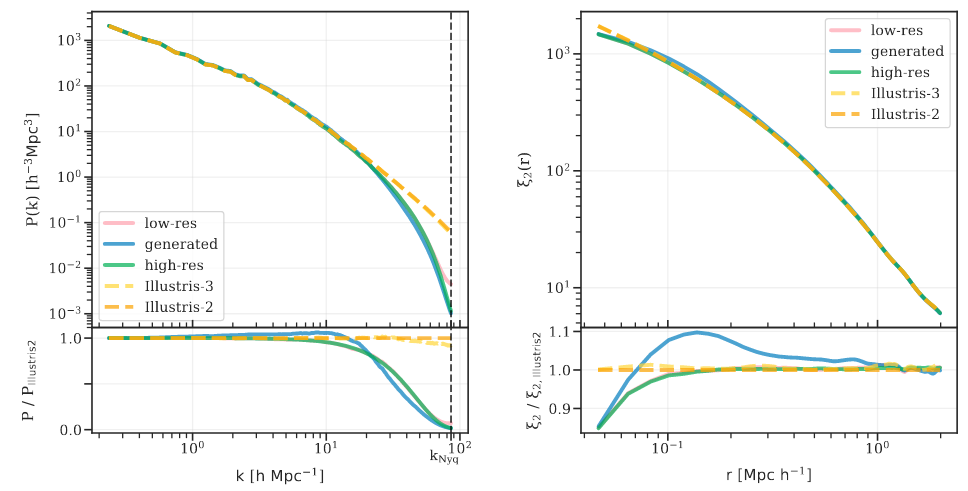
\includegraphics[width=\textwidth]{power-spectrum.png}
  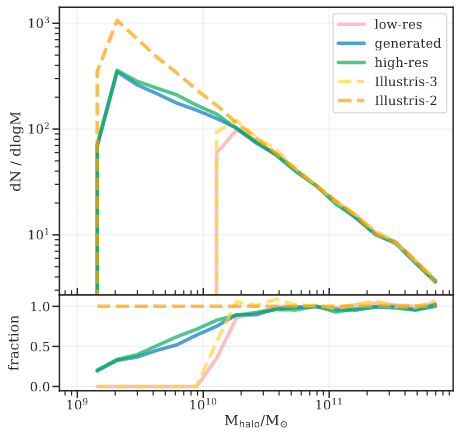
\includegraphics[width=0.45\textwidth]{halo-mass.png}
  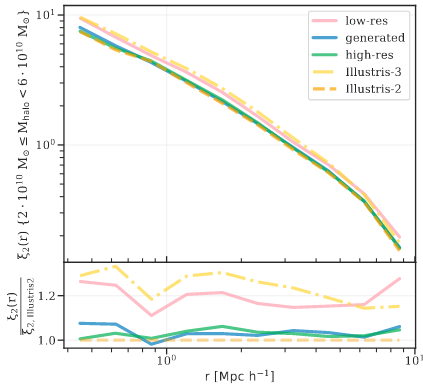
\includegraphics[width=0.45\textwidth]{halo-correlation.png}
  \caption{These are figure 4, 5, and 6 from \cite{superresolving-halos}. I will try to replicate it with Enzo in place of Illustris}
  \label{Illustris-fig}
\end{figure}
